\documentclass{beamer}
\usepackage{pgfpages}
\usepackage[backend=bibtex]{biblatex}
\usepackage{multicol}
\usepackage{multimedia}
\usepackage[absolute,overlay]{textpos}
\usepackage{parskip}
\usepackage{hyperref}
\usepackage{lmodern}
\usepackage{bbding}
\usepackage[absolute,overlay]{textpos}
\usepackage{framed} %Used to shade important equations, color devined with shadecolor
\hypersetup{colorlinks=true, urlcolor=blue}
\setlength{\parskip}{\smallskipamount}
\colorlet{shadecolor}{cyan}
%\usepackage[texcoord,grid,gridunit=mm,gridcolor=red!10,subgridcolor=green!10]{eso-pic} %DELETE when done with grid
\setbeameroption{hide notes} % Only slides
%\setbeameroption{show only notes} % Only notes
%\setbeameroption{show notes on second screen=right} % Both
%\bibliography{../../papers/references.bib}
\setbeamerfont{footnote}{size=\tiny}
%\AtEveryCitekey{\clearfield{title}}

%
% Choose how your presentation looks.
%
% For more themes, color themes and font themes, see:
% http://deic.uab.es/~iblanes/beamer_gallery/index_by_theme.html
%
\mode<presentation>
{
\usetheme{Warsaw}      % or try Darmstadt, Madrid, Warsaw, ...
\usecolortheme{default} % or try albatross, beaver, crane, ...
\usefonttheme{default}  % or try serif, structurebold, ...
\setbeamertemplate{navigation symbols}{}
\setbeamertemplate{caption}[numbered]
} 

\usepackage[english]{babel}
%\usepackage[utf8x]{inputenc} %Doesn't play well with biblatex
\usepackage{amssymb}
\usepackage{bm}
\usepackage{color}
\usepackage{graphicx}
\setbeamercovered{invisible}
\setbeamercovered{%
again covered={\opaqueness<1->{100}}} %This changes the opaqueness of each bullet

\newcommand{\red}[1]{{\color{red}{#1}}}
\newcommand{\checkH}[2]{\begin{textblock*}{1cm}(#1,#2){\Huge \red{\Checkmark}}\end{textblock*}}
\newcommand{\checkh}[2]{\begin{textblock*}{1cm}(#1,#2){\huge \red{\Checkmark}}\end{textblock*}}
\newcommand{\checkL}[2]{\begin{textblock*}{1cm}(#1,#2){\Large \red{\Checkmark}}\end{textblock*}}
\newcommand{\checkl}[2]{\begin{textblock*}{1cm}(#1,#2){\large \red{\Checkmark}}\end{textblock*}}
\renewcommand{\rm}[1]{\mathrm{#1}}

\title[{\color{white}{Chapters 3}}]{Physics 121: \\ Vectors and Coordinate Systems}
\author{Cody Petrie}
\institute{Mesa Community College}
\date{}

\begin{document}

%\setbeamertemplate{frametitle}[default][center]
\begin{frame}
\titlepage
\end{frame}

% Uncomment these lines for an automatically generated outline.
%\begin{frame}{Outline}
%  \tableofcontents
%\end{frame}

% Commands to include a figure:
%\begin{figure}
%\includegraphics[width=\textwidth]{your-figure's-file-name}
%\caption{\label{fig:your-figure}Caption goes here.}
%\end{figure}

\begin{frame}{Quiz}
\begin{enumerate}
   \item What is the magnitude of the gravitational acceleration near the surface of the earth?
   \begin{columns}
      \begin{column}{0.5\textwidth}
      \begin{enumerate}
         \item[A.] 4.98 m/s$^2$
         \item[C.] 9.80 m/s$^2$
      \end{enumerate}
      \end{column}
      \begin{column}{0.5\textwidth}
      \begin{enumerate}
         \item[B.] 9.80 m/s
         \item[D.] It depends on the velocity
      \end{enumerate}
      \end{column}
   \end{columns}
~\\~\\
   \item Which of these is {\bf NOT} a kinematic equation?
   \begin{columns}
      \begin{column}{0.5\textwidth}
      \begin{enumerate}
         \item[A.] $s_f = s_i + v_i\Delta t + \frac{1}{2}a(\Delta t)^2$
         \item[C.] $a_f = a_i + \int\limits_{t_i}^{t_f} v_sdt$
      \end{enumerate}
      \end{column}
      \begin{column}{0.5\textwidth}
      \begin{enumerate}
         \item[B.] $v_f = v_i + a\Delta t$
         \item[D.] $v_f^2 = v_i^2 + 2a\Delta s$
      \end{enumerate}
      \end{column}
   \end{columns}
\end{enumerate}
\end{frame}

\begin{frame}{Reminders}
\begin{itemize}
   \item The next HW will be due on Saturday and will include all the material we cover in chapters 3 and 4.
   \item The exam is coming up on Tuesday 19 Sep. The exam will be taken in class. It will cover all material from chapters 1-4.
\end{itemize}
\end{frame}

\begin{frame}{Vectors}
\begin{center}
   Before we dive anymore into physics and motion in multiple dimensions let's do a thorough review of vectors!
\end{center}
\end{frame}

\begin{frame}{Vectors}
\begin{itemize}
   \item<1-> In your words what is a vector?
   \item<2-> You have learned how to add vectors as pictures so I won't bore you with that.
   \begin{center}
      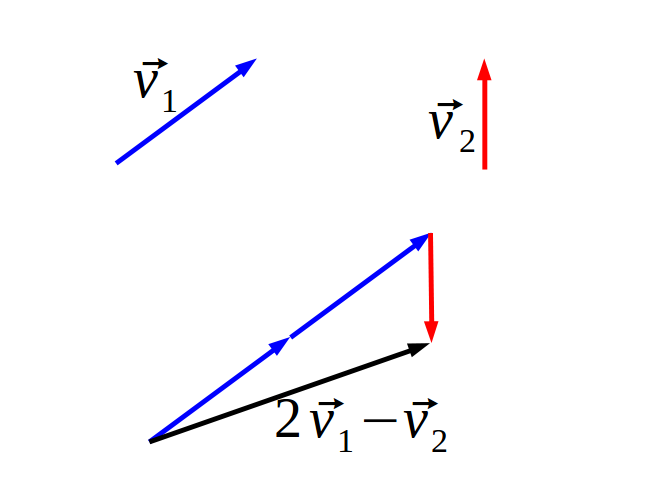
\includegraphics[width=0.5\textwidth]{../figures/1_4-5QuizAns.png}
   \end{center}
   \item<3-> However we haven't talked about their components in detail much.
\end{itemize}
\end{frame}

\begin{frame}{Vectors}
\begin{center}
   Write down how you would describe this vector
   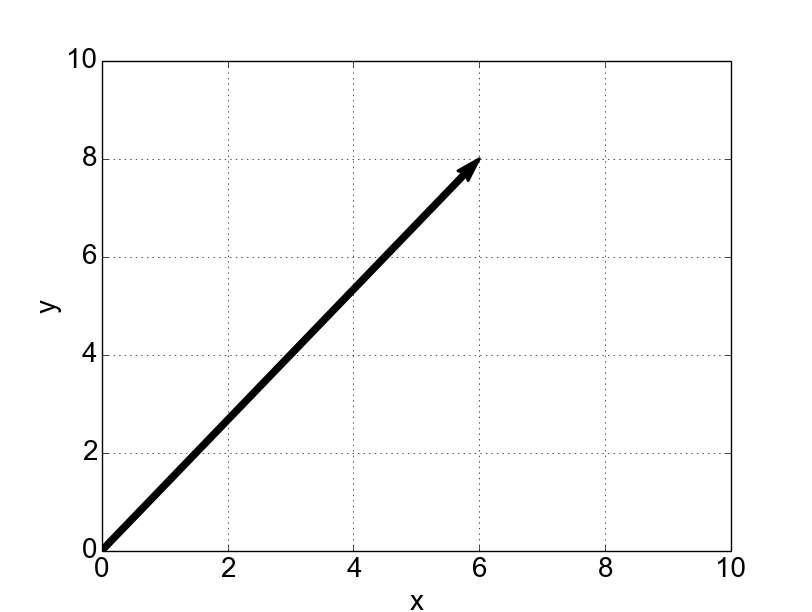
\includegraphics[width=0.9\textwidth]{../figures/vec_chap3.png}
\end{center}
\end{frame}

\begin{frame}{Vectors}
\begin{center}
   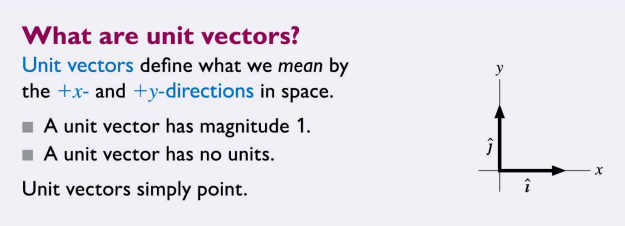
\includegraphics[width=0.9\textwidth]{../figures/3_unitvector.png}
\end{center}
\end{frame}

\begin{frame}{Vectors}
\begin{itemize}
   \item<1-> What is the difference between a scalar and a vector?
   \item<2-> The magnitude (length) of a vector is a scalar (ex. $\vec{V}=X\hat{i}+Y\hat{j}$).
   \begin{equation*}
      V=\left|\vec{V}\right| = \sqrt{X^2+Y^2}
   \end{equation*}
   Think of the pythagorean theorem
   \item<3-> If the vector was the velocity then notice that the magnitude would be the speed. Also, the magnitude cannot be negative (just like speed can't be negative, but velocity can).
\end{itemize}
\end{frame}

\begin{frame}{Vectors}
\begin{center}
   Add the two displacement vectors, $\vec{A}$ and $\vec{B}$ to get the {\bf resultant vector} (or total displacement) $\vec{C}$. \\~\\
   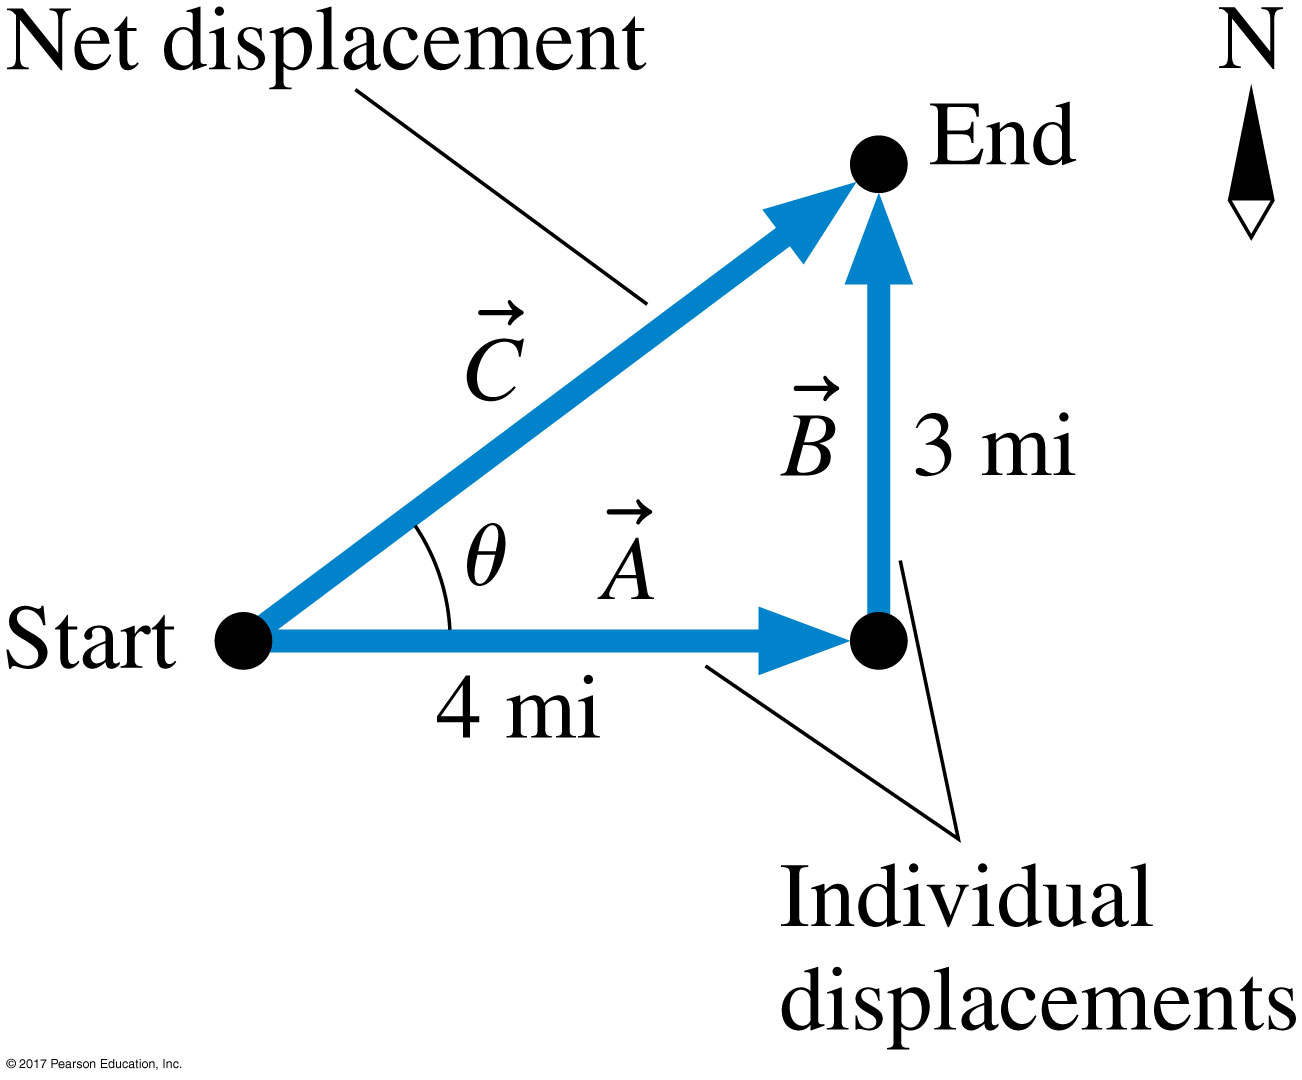
\includegraphics[width=0.5\textwidth]{../figures/03_03_Figure.jpg}
   \uncover<2>{\\~\\ $\vec{C}$ = 4 mi $\hat{i} + $ 3 mi $\hat{j}$}
\end{center}
\end{frame}

\begin{frame}{Vectors}
\begin{center}
   This time use $\vec{A}$ and $\vec{B}$ to get $\vec{C}$ in terms of the magnitude $C$ and the angle as measured from the x axis, $\theta$. \\~\\
   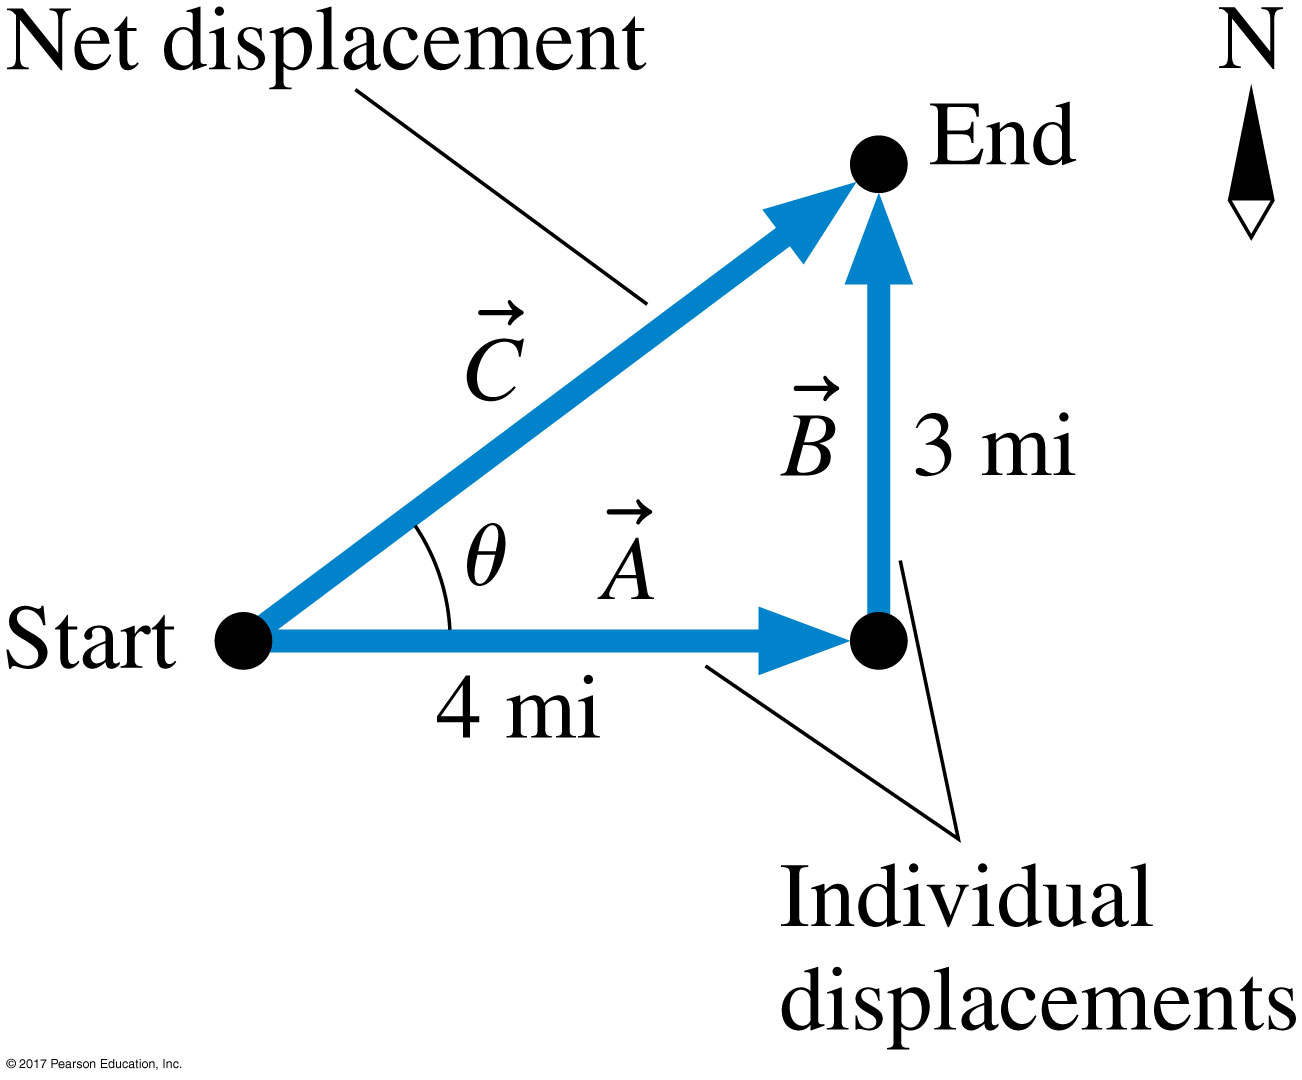
\includegraphics[width=0.5\textwidth]{../figures/03_03_Figure.jpg}
   \uncover<2>{\\~\\ $C = \sqrt{A^2+B^2} = \sqrt{(4 \text{ mi})^2 + (3 \text{ mi})^2} =$ 5 mi \\ $\theta = \tan^{-1}\left(\frac{B}{A}\right) = \tan^{-1}\left(\frac{3 \text{ mi}}{4 \text{ mi}}\right) = 37 ^\circ$}
\end{center}
\end{frame}

\begin{frame}{Quick Check}
\begin{center}
   What is $\vec{A}_1 + \vec{A}_2 + \vec{A}_3$?
   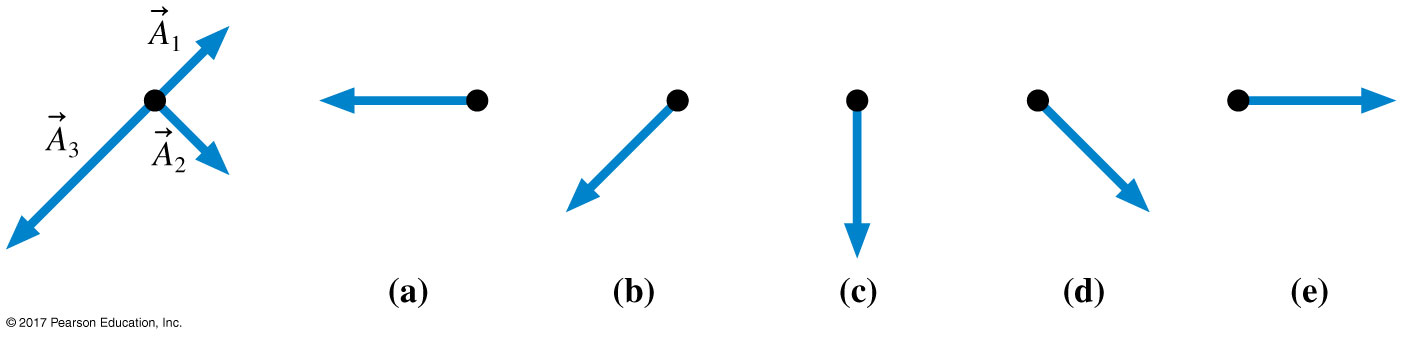
\includegraphics[width=\textwidth]{../figures/Figure_STT3_1.jpg}
   \only<2->{\checkL{7.2cm}{5.8cm}}
\end{center}
\end{frame}

\begin{frame}{Quick Check}
\begin{center}
   Which figure shows $2\vec{A}-\vec{B}$?
   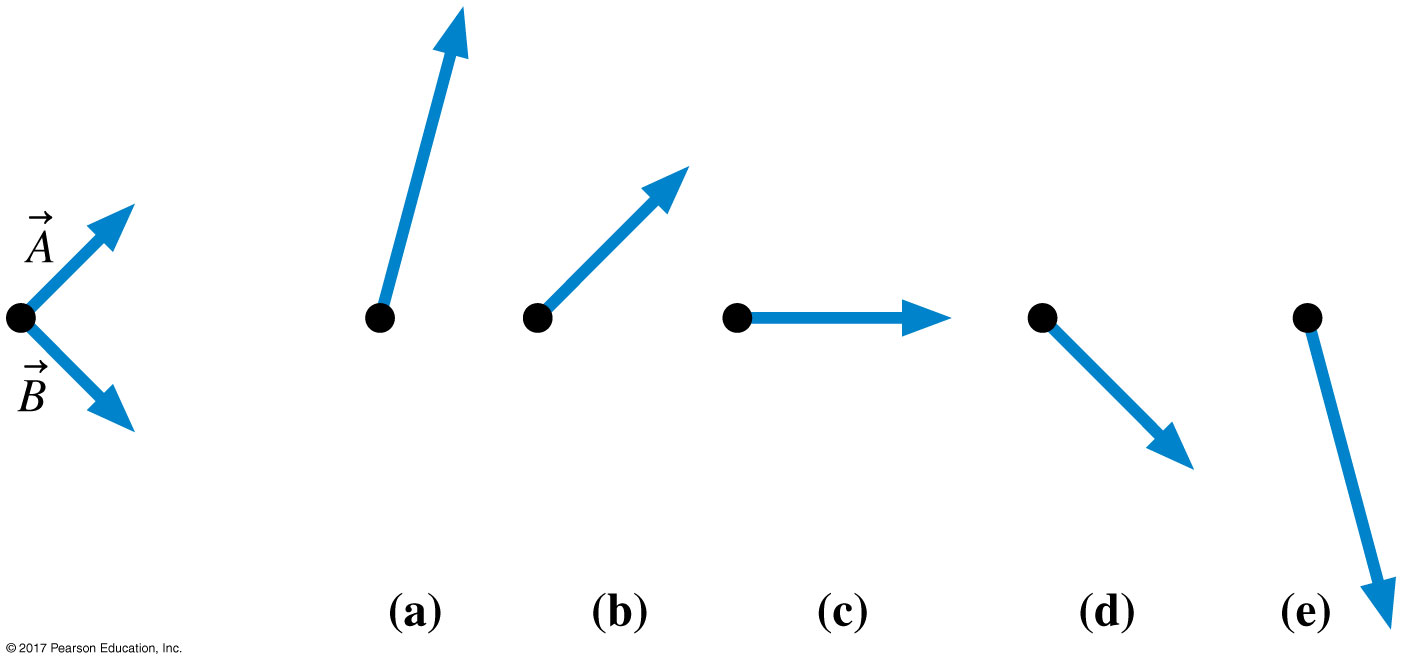
\includegraphics[width=\textwidth]{../figures/Figure_STT3_2.jpg}
   \only<2->{\checkL{3.8cm}{7.3cm}}
\end{center}
\end{frame}

\begin{frame}{Vectors}
\begin{center}
   More vector math \\~\\
   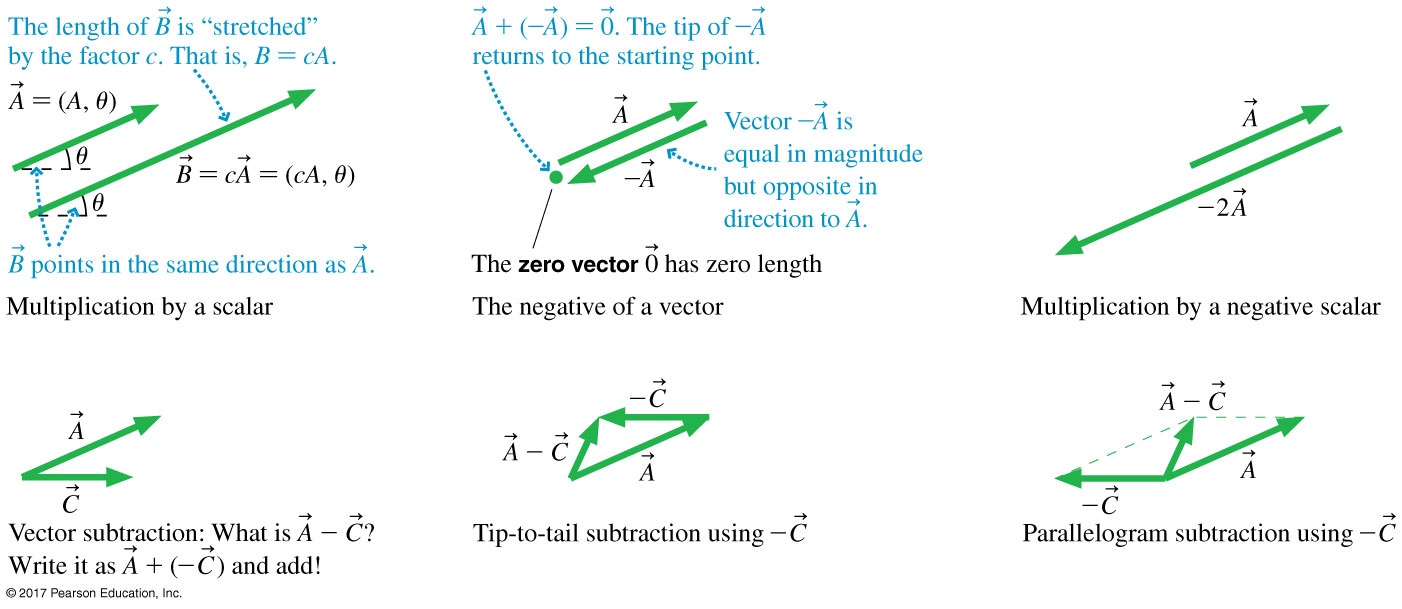
\includegraphics[width=\textwidth]{../figures/03_07_Figure.jpg}
\end{center}
\end{frame}

\begin{frame}{Coordinate Systems}
\begin{itemize}
   \item We have talked about coordinate systems and origins (on the first day)
   \item Which of these things depends on the coordinate system and origin?
   \begin{enumerate}
      \item Vector components
      \item Magnitude of vector
      \item Angle of vector
      \item Displacement vector (i.e. $\Delta \vec{r} = \vec{r}_1 - \vec{r}_0$)
   \end{enumerate}
\end{itemize}
\begin{center}
   \uncover<2>{1 and 3}
\end{center}
\end{frame}

\begin{frame}{Coordinate Systems}
\begin{itemize}
   \item Once we have picked a suitable coordinate system we can then take any vector and decompose it into it's {\bf component vectors}. This is called {\bf decomposition} of a vector into it's component vectors.
   \begin{center}
      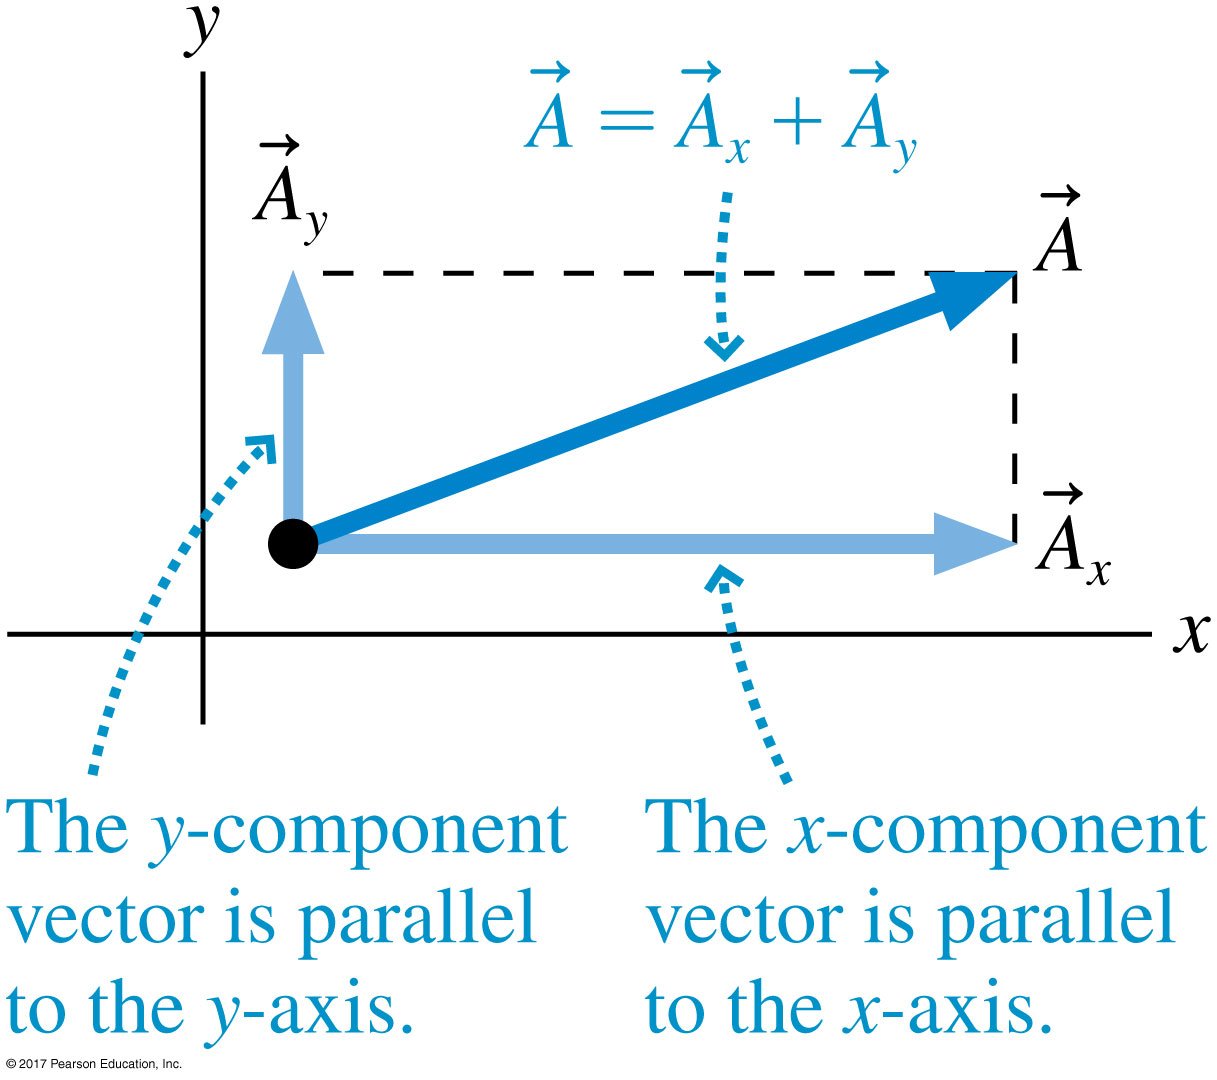
\includegraphics[width=0.6\textwidth]{../figures/03_10_Figure.jpg}
   \end{center}
\end{itemize}
\end{frame}

\begin{frame}{Warning}
\begin{center}
   Just as a warning $\vec{A}_x$ is not the same as the component $A_x$. $\vec{A}_x = A_x \hat{i}$.
\end{center}
\end{frame}

\begin{frame}{Warning \#2}
\begin{center}
   As a second warning when going between component and geometric forms of vectors make sure you get signs right (sometimes you have to put them in by hand) and make sure you know where angles are being measured from. \\
   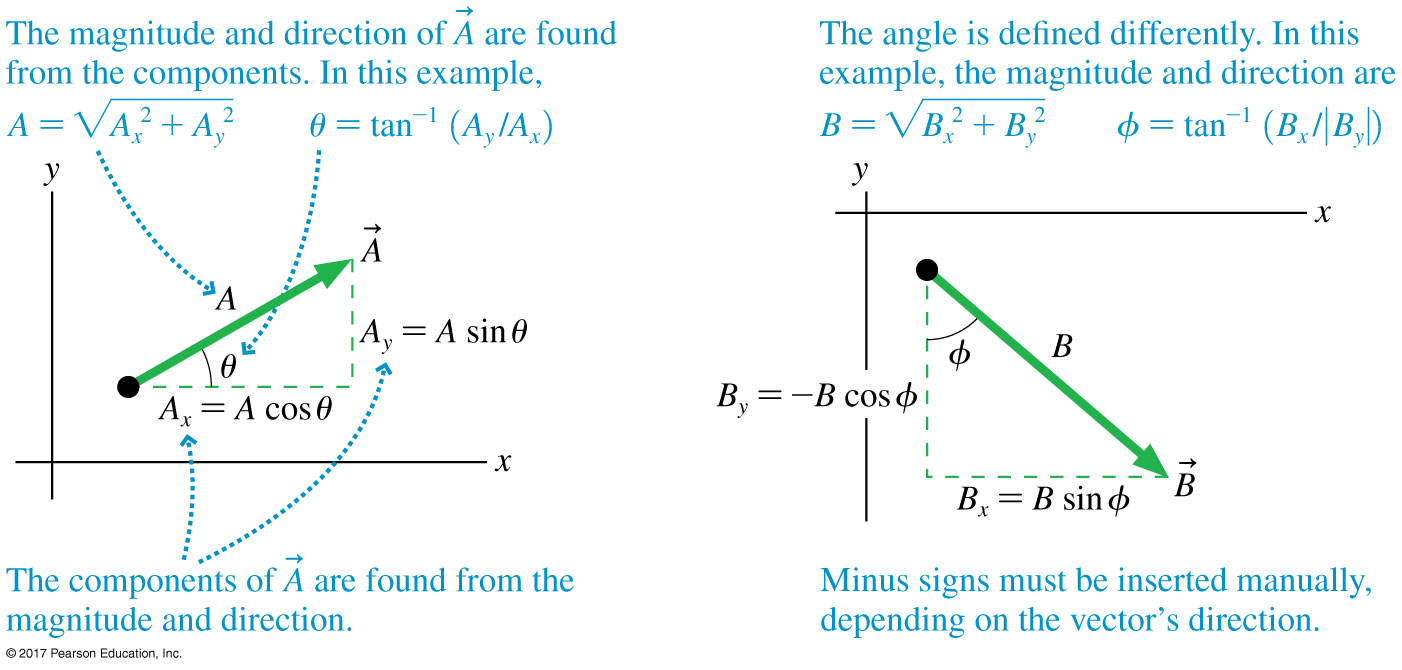
\includegraphics[width=\textwidth]{../figures/03_12_Figure.jpg}
\end{center}
\end{frame}

\begin{frame}{Quick Check}
\begin{center}
   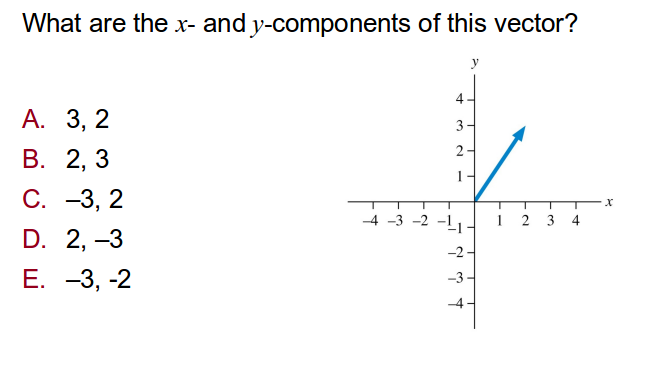
\includegraphics[width=\textwidth]{../figures/QC3_3.png}
\end{center}
\only<2->{\checkL{1.0cm}{3.8cm}}
\end{frame}

\begin{frame}{Quick Check}
\begin{center}
   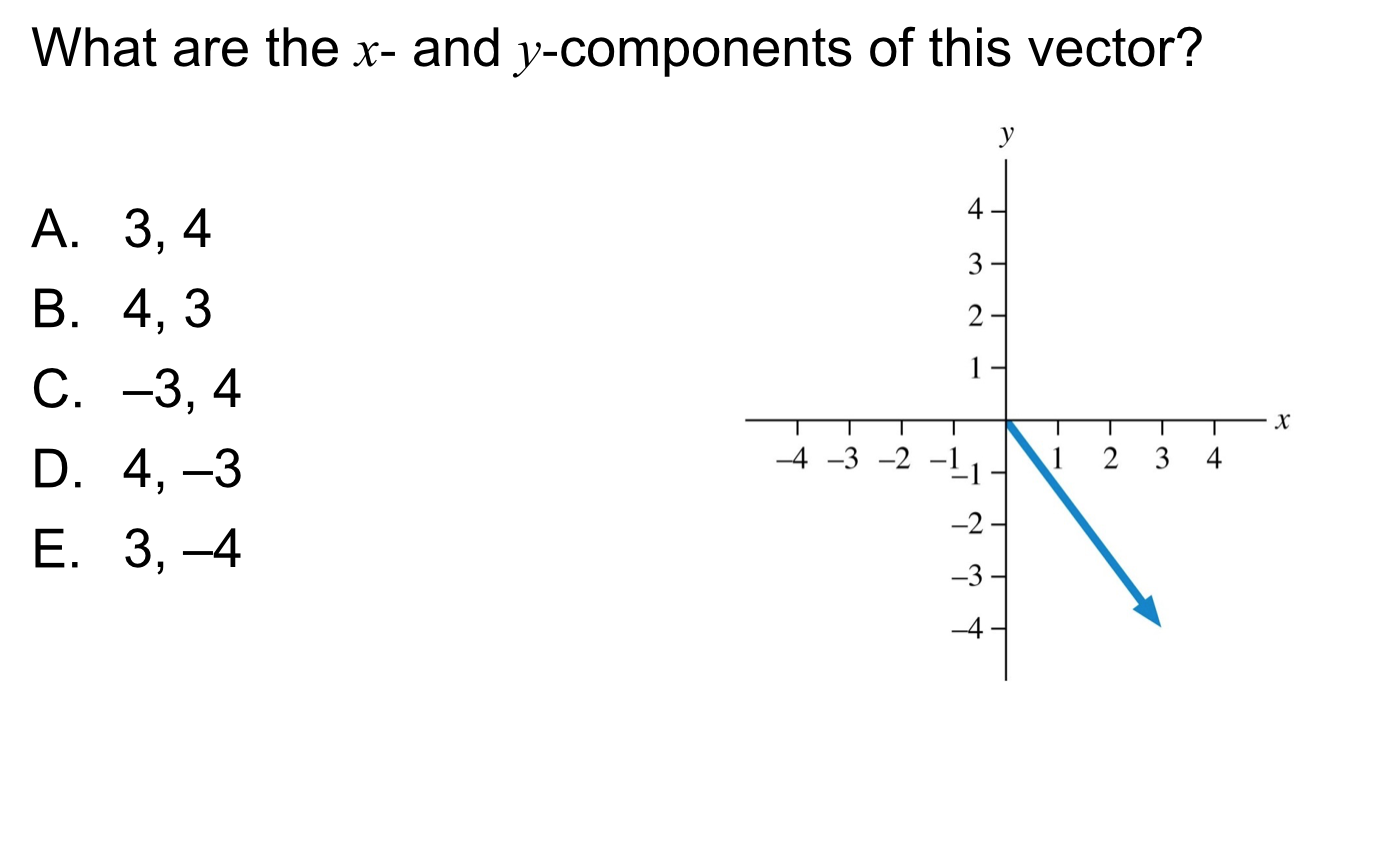
\includegraphics[width=\textwidth]{../figures/QC3_4.png}
\end{center}
\only<2->{\checkL{0.9cm}{5.4cm}}
\end{frame}

\begin{frame}{Quick Check}
\begin{center}
   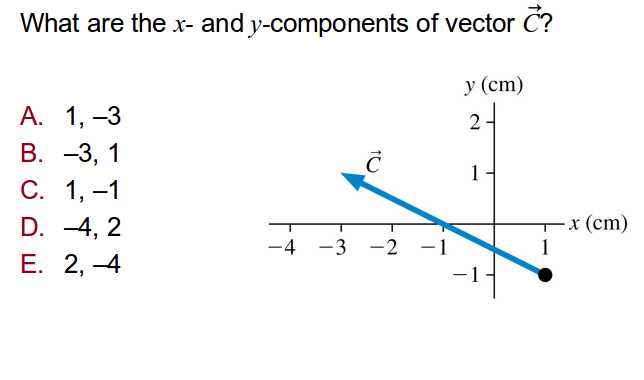
\includegraphics[width=\textwidth]{../figures/QC3_5.png}
\end{center}
\only<2->{\checkL{1.0cm}{5.0cm}}
\end{frame}

\begin{frame}{Vector Math}
\begin{itemize}
   \item How would you add three vectors $\vec{D}=\vec{A}+\vec{B}+\vec{C}$ where the vectors are given by $\vec{A} = A_x\hat{i} + A_y\hat{j}$ and similar for $\vec{B}$ and $\vec{C}$?
   \uncover<2>{
      $\vec{D}=(A_x+B_x+C_x)\hat{i}+(A_y+B_y+C_y)\hat{j}$
   }
\end{itemize}
\end{frame}

\begin{frame}{Quick Check}
\begin{center}
   A bird flies 100 m due east from a tree, then 50 m northwest ($45^\circ$ north of west). What is the bird
s net displacement?
   \uncover<2>{
      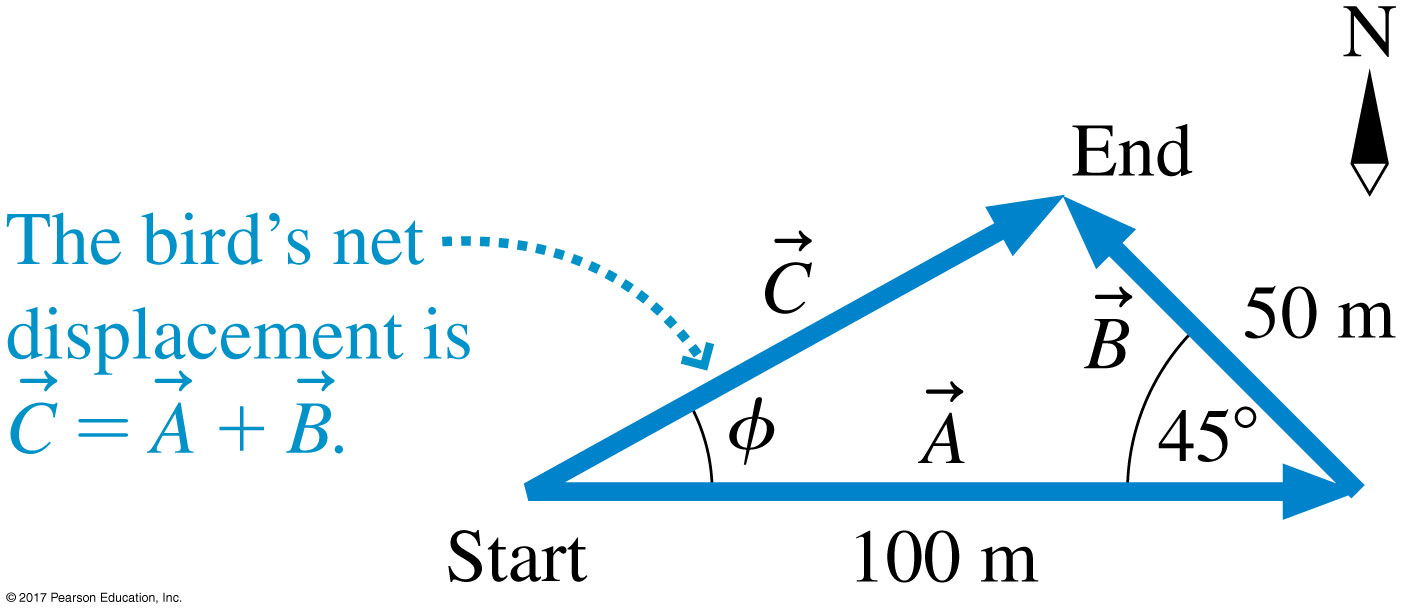
\includegraphics[width=0.5\textwidth]{../figures/03_04_Figure.jpg}
      \\ $\vec{A} = 100\hat{i}$ \\
      $\vec{B} = -50\sin(45^\circ) \hat{i} + 50\sin(45^\circ) \hat{j} = -35.4\hat{i} + 35.4\hat{j}$ \\
      \red{$\vec{C} = 64.6\hat{i} + 35.4\hat{j}$}\\
   }
   \uncover<3>{
      $C=\sqrt{C_x^2+C_y^2} = \sqrt{64.6^2 + 35.4^2} = 73.6 m$ \\
      $\theta = \tan^{-1}\left(\frac{C_y}{C_x}\right)\tan^{-1}\left(\frac{35.4}{64.6}\right) = 28.7^\circ$\\
      \red{$\vec{C} = (73.6 \text{ m}, 28.7^\circ)$}
   }
\end{center}
\end{frame}

\begin{frame}{Tilted Axes}
\begin{itemize}
   \item Let's say I have an inclined plane. Can I set my axes such that $\hat{i}$ points along (parallel) to the plane and $\hat{j}$ points perpendicular to the plane?
   \item<2-> Of course you can, we talked about how that could be useful last time! This can help you determine the component vectors that are ``parallel" (make object move) and ``perpendicular" (doesn't make the object move).
   \begin{center}
      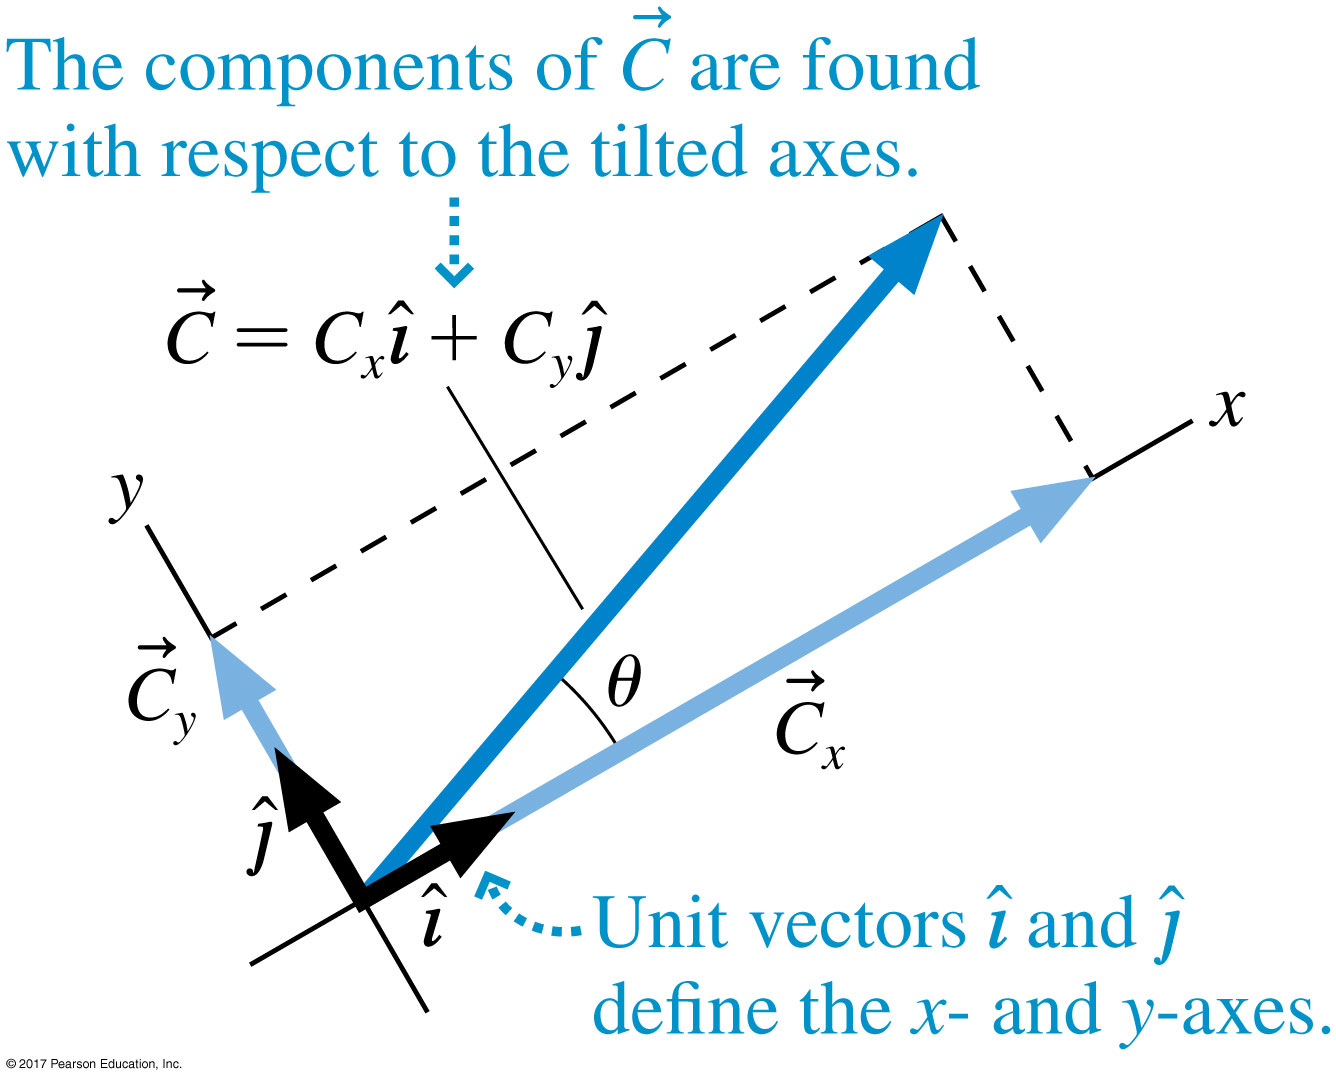
\includegraphics[width=0.5\textwidth]{../figures/03_20_Figure.jpg}
   \end{center}
\end{itemize}
\end{frame}

\begin{frame}{Tilted Axes}
\begin{center}
   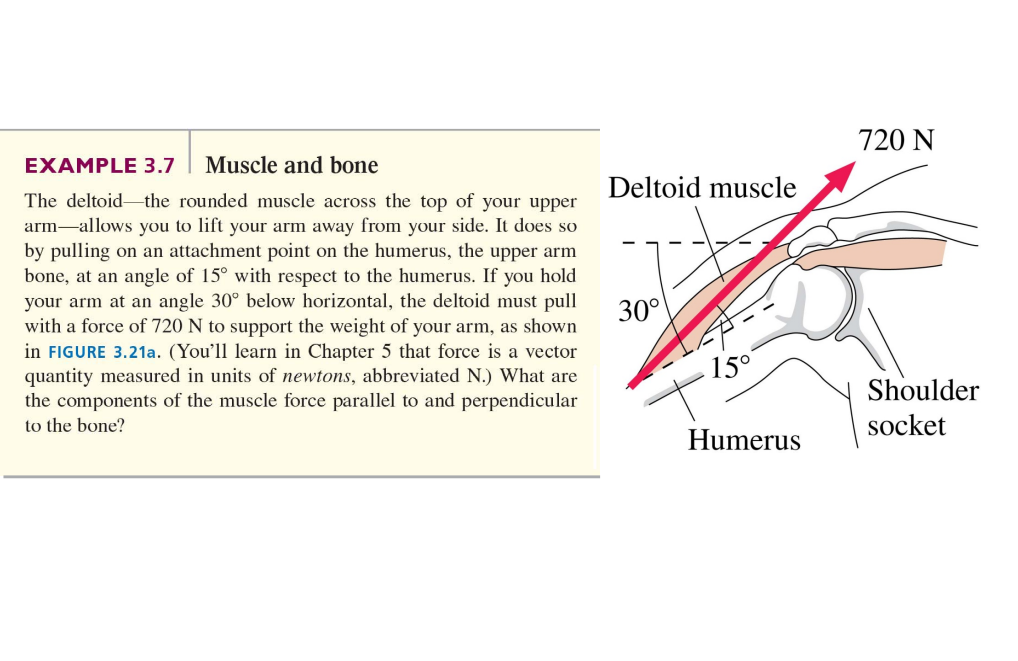
\includegraphics[width=\textwidth]{../figures/Ex3_7-1.png}
\end{center}
\end{frame}

\begin{frame}{Tilted Axes}
\begin{center}
   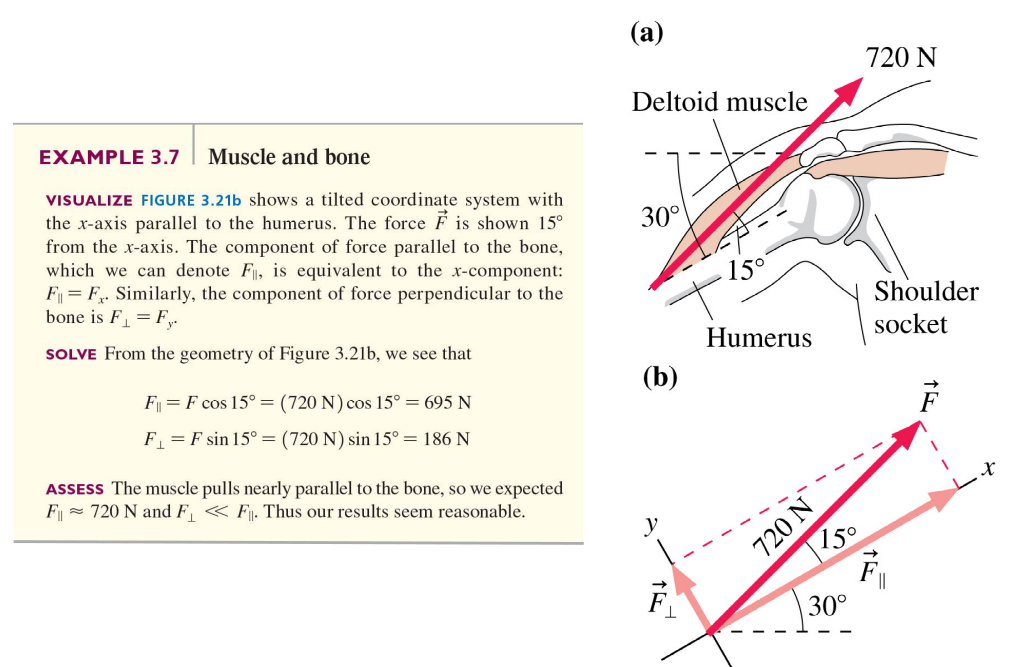
\includegraphics[width=\textwidth]{../figures/Ex3_7-2.png}
\end{center}
\end{frame}

\begin{frame}{Picture References}
\tiny
None yet
\end{frame}

\end{document}
